\documentclass{article}
\usepackage{amsmath}
\usepackage{amssymb}
\usepackage{graphicx}
\usepackage{hyperref}
\usepackage[version=4]{mhchem}

\title{Example 5}
\date{}

\begin{document}
\maketitle

(2002 AMC 10A Problem 25) In trapezoid \(A B C D\) with bases \(A B\) and \(C D\), we have \(A B=52, B C=12, C D=39\), and \(D A=5\). The area of \(A B C D\) is\\
(A) 182\\
(B) 195\\
(C) 210\\
(D) 234\\
(E) 260\\
\centering
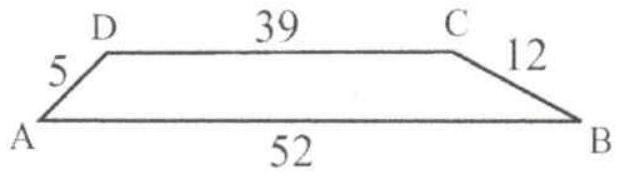
\includegraphics[width=\textwidth]{images/077(1).jpg}

Solution: (C).\\
Method 1:\\
First drop perpendiculars from \(D\) and \(C\) to \(A B\). Let \(E\) and \(F\) be the feet of the perpendiculars to \(A B\) from \(D\) and \(C\), respectively, and let \(h=D E=C F, x=A E\), and \(y=F B\).\\
\centering
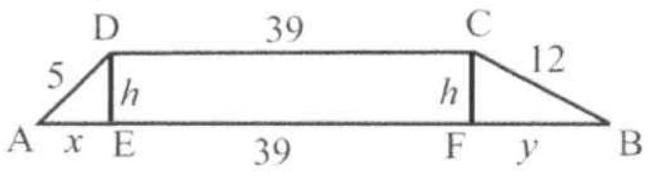
\includegraphics[width=\textwidth]{images/077.jpg}\\
\(25=h^{2}+x^{2}, 144=h^{2}+y^{2}\) and \(13=x+y\)\\
So\\
\(144=h^{2}+y^{2}=h^{2}+(13-x)^{2}=h^{2}+x^{2}+169-26 x=25+169-26 x\), which gives \(x=\frac{50}{26}=\frac{25}{13}\), and \(h=\sqrt{5^{2}-\left(\frac{25}{13}\right)^{2}}=5 \sqrt{1-\frac{25}{169}}=5 \sqrt{\frac{144}{169}}=\frac{60}{13}\).


Hence Area of \(A B C D=\frac{1}{2}(39+52) \times \frac{60}{13}=210\).

Method 2:\\
First drop perpendiculars from \(D\) and \(C\) to \(A B\). Let \(E\) and \(F\) be the feet of the perpendiculars to \(A B\) from \(D\) and \(C\), respectively, and let \(h=D E=C F, x=A E\), and \(y=F B\).\\
\centering
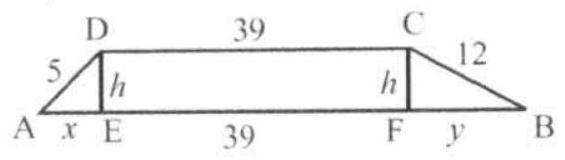
\includegraphics[width=\textwidth]{images/078(1).jpg}

By the Pythagorean Theorem, we have:\\
\(h^{2}=5^{2}-x^{2}=12^{2}-y^{2} \Rightarrow y^{2}-x^{2}=12^{2}-5^{2}=119\)\\
We know that \(y+x=52-39=13\).

Therefore (1) becomes\\
\((y-x)(y+x)=119 \Rightarrow 13(y-x)=119 \quad \Rightarrow y-x=\frac{119}{13}\)\\
Solving the system of equations (2) and (3), we get \(x=\frac{25}{13}\).\\
Therefore \(h^{2}=5^{2}-x^{2}=25-\frac{5}{13} \quad \Rightarrow \quad h=\frac{60}{13}\).\\
The area of \(A B C D\) is then \(\frac{39+52}{2} \times \frac{60}{13}=210\).\\

\end{document}
